\section{Client}

This section will analyse how appropriate our client design was to achieve the aims outlined in section \ref{client_design}. Some of our design choices worked well, such as the interfaces used by the controller to separate concerns. Another decision that worked well was our use of the object oriented features of Java to implement chat windows, which reduced the challenge of routing internal messages to the correct windows. These aspects will be discussed in section \ref{designimpl}.

While implementing the client, it became clear that some of our larger design choices were na\"{\i}ve, and further design work had to be conducted. One case involved the interaction between the controller and networking subsystem. These changes will be discussed in section \ref{designimpl}. In some cases, smaller design choices required larger changes. Of particular significance, our understanding of the practical working of the GIM protocol to create personal chats proved to be weak. This required design work reaching over the protocol and the model component of the system. This process tested our ability to collaborate as a team to implement an interacting system. The degree of success of our changes will be discussed in section \ref{collab}. Furthermore, as we became more familiar with the Java Swing environment, our code went through evolutionary steps to implement certain features in a more sensible manner, such as how displaying updates to user information was handled. Section \ref{code_evol} will discuss problems we identified with code that was functional but deemed to be hard to maintain, and the merits of the changes we made, such as in the above case.

\subsection{Design Implementation}
\label{designimpl}

\begin{figure}
    \begin{center}
        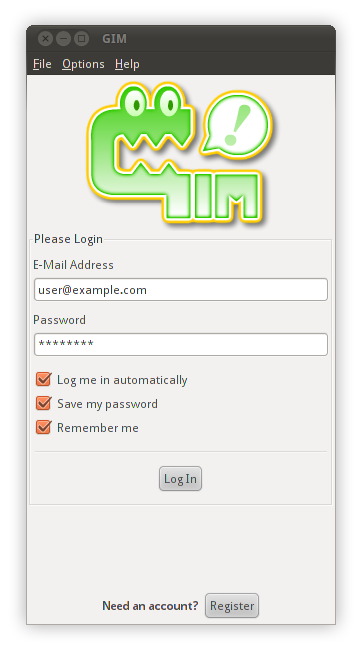
\includegraphics[scale=0.6]{Implementation/diagrams/login.png}
        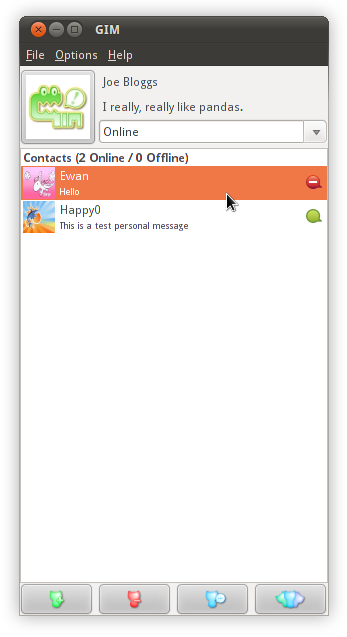
\includegraphics[scale=0.6]{Implementation/diagrams/main.png}
        \caption{The login panel and main window of the GIM Client}
        \label{MainWindowDia}
    \end{center}
\end{figure}

In the design section we outlined how we envisioned the flow of information between the controller and networking components would work. When we started coding the controller component, it became clear that it would be more sensible for it to be made up of multiple classes. In our design, we thought the controller would be made up of one class, which implemented the two interfaces created in the design stage. These interfaces would handle incoming and outgoing commands in the GIM protocol. However, as we began writing method stubs, our controller class looked bloated, and incorporated too many responsibilities. Instead, we created two classes: one to handle events for outgoing traffic, and one to handle incoming traffic, implementing the `networkingOut' and `networkingIn' interfaces respectively.

To create the networking component, the client had to create an instance of the ClientConnection class and pass the network a ServerConnection object. It used this object to call methods after receiving commands from the server. There is a further difference here from our design. Our original plan was to have the controller thread waiting until a buffer between the networking component and controller component had a new message from the server. This thread would then parse it and call a method within the controller. However, as our understanding of threading progressed, we realised that this plan would not work as the interface can only be accessed from the GUI thread. After some confusion attempting to implement our ill informed design, we had to investigate an alternative method of altering the GUI. Upon further learning of concurrency in Swing, we discovered that Swing has a `buffer' (named the ``Event Queue'') of its own, that could be used as an alternative to queue GUI events.\footnote{See http://www.kauss.org/Stephan/swing/index.html for a more detailed discussion of the Swing Event Queue.} To use this event queue, it is necessary to wrap any code you wish to run on the GUI thread in an anonymous class implementing a method called Runnable as a parameter to the invokeLater method.  While it would be possible to read commands off our own buffer, and then buffer alterations to the GUI in to event queue, we thought this would be redundant behaviour as there would then be two intermediate queues. Instead, we decided the appropriate method would be called directly from the network reader, and the event queue would be used where it was necessary to alter the interface.

In retrospect, we may have abused this option in our implementation. There are some operations we add to the Swing Event Queue that do not effect the interface. In some cases, this is necessary as some information has to be changed in order to keep operations sequential. However, there are some cases where it is not clear if operations need to be run on the event queue. Furthermore, in some cases our program appeared to working as expected, except in some fringe cases. After much work, we found we had not wrapped code that needed to be synchronized in the event queue. A possible alternative would be to have used our original plan of reading commands from the buffer, parsing them in the controller, and calling the appropriate method. Since most almost all commands from the server effect the GUI, all method calls could have been wrapped in the event queue at this stage. This would have served to have kept our code tidier (as the event queue would only be used once), and have inherently solved many of the threading problems we had by not invoking the event queue. As we only incrementally became aware of methods that required the event queue, it is clear we did not have a full understanding of the problems of threading in the early stages. By tackling this project, we have since learned the need for more careful consideration of threading issues.

In the section \ref{networking_design}, we outlined how we believed commands from the server would be parsed. While the operations of the proposed Command class remained largely intact, its responsibility of parsing had to be removed. Our original plan that this feature could be shared by the client and the server wasn't possible, as it was apparent that the server had some responsibilities with parsing that the client did not. It had to ensure that it was not receiving too many commands within a time frame, and that these commands were of a limitted length. These limits do not apply to the client, as it is allowed to receive large amounts of data from the server, such as the user information for the buddy list (which may be long).

\begin{figure}
    \begin{center}
        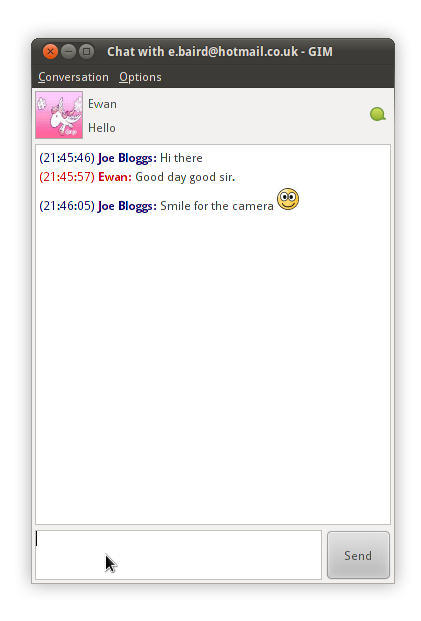
\includegraphics[scale=0.5]{Implementation/diagrams/single_chat.png}
        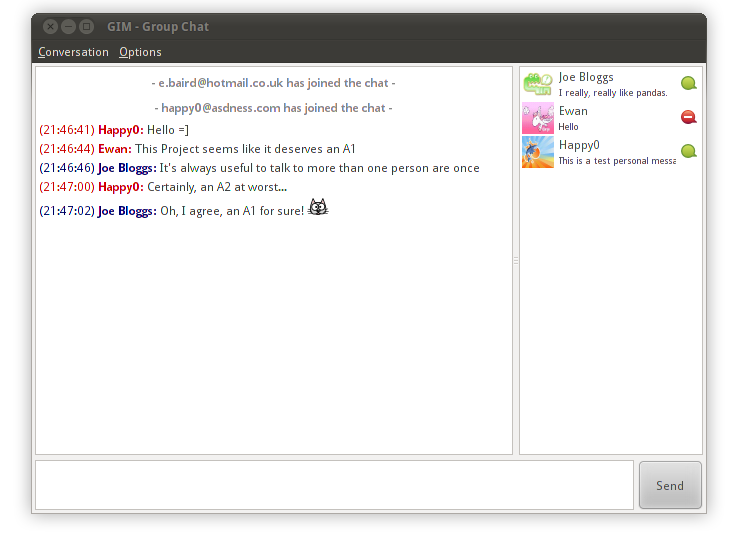
\includegraphics[scale=0.5]{Implementation/diagrams/group_chat.png}
        \caption{Examples of single and group chat windows in GIM.}
        \label{MainWindowDia}
    \end{center}
\end{figure}

\subsection{Collaboration}
\label{collab}

The first draft of the GIM protocol treated all conversations as `rooms' and did not distinguish group chats and personal chats (Rooms were discussed in section \ref{message_routing}). In designing the protocol, we wished to keep it abstract and not fall into the trap of implicitly implementing features that the client and server could handle. Our goal was not to develop a protocol suitable for only one type of implementation. Originally, it was believed that the client could distinguish personal chats and group chats by storing internal records of the type of outgoing invites to chat. In the case of being invited to chat, we believed using the protocol's \texttt{USER} argument in the \texttt{:ROOM:} command would be sufficient to count the amount of users in the room and determine the type of chat. However, as we began implementing room creation, it became clear that the initial group user list could be of size 1, and thus the wrong chat window could be created. As a result, the protocol had to be changed, and the client amended to reflect these changes. 

This change was a test of the boundary of responsibilities within our system, as it effected communication with the server and the back end of the client. The protocol engineer's solution to the issue was to add a `type' argument to the room command. In the case creating a room, the type now had to be specified. To allow a user to work out what room type a chat had, the `type' argument would be used, with a room identifier. This kept the protocol more abstract. In order to deal with these changes, our client had to be designed to sequence responses from the server for certain requests. As the protocol did not include sequence numbers, we had to re-design the model to perform this task. It was apparent that the amount of talk between the client and server required to start a chat was now increased. This required an understanding of what needed to be achieved at each stage in the conversation. This high level plan was determined:

Creation:
\begin{enumerate}
\item Client adds the type of room to be created to the new room queue in the model.
\item Client notes a list of user(s) invited to chat in the invitations queue in the model.
\item Client sends request to server to create a room of this type.
\item Server responds with `created' and the room id.
\item Client matches the type of chat with the `new room' queue, and the user list from the `invitations' queue.
\item Client spawns the appropriate chat window (and adds to the list of chat windows), or updates the internal state information of an existing window in the window list, associated with the participant. Information includes who is in the room and the id to send messages to.
\item Client is informed that the participant has joined the room, through the \texttt{JOINED} argument in the \texttt{:ROOM:} command.
\end {enumerate}

Invitation:
\begin{enumerate}
\item Client receives invite to chat from server with certain room id from user. Store username in an `invited' queue in model.  
\item Client asks server the type of the room that it has been invited to.
\item Server responds with `Personal' or `Group.'
\item Client matches request with response from the `invited' queue.
\item Client spawns the appropriate chat window (and adds to the list of chat windows), or updates the internal state information of an existing window, in the window list, associated with the participant. Information includes who is in the room and the id to send messages to.
\item Client is informed that the participant has joined the room, through the \texttt{JOINED} argument in the \texttt{:ROOM:} command.
\item If it is a group chat, client asks server for the user list in the room.
\end{enumerate}

In retrospect, the trade off between keeping an abstract protocol--which could be used for different styles of implementation--and designing towards our own client and server may have been too high. Aside from the communication between the client and the server, there are complexities within the client code to ensure these events are performed in sequence which left much opportunity for error in the control of threading. For example, a user should not be allowed to send a message before the conversation participant has also joined the room, in the case of a personal chat between steps 6 and 7 (in the ``Creation'' plan). This meant that safeguards had to be considered during this sequence of events to make sure messages were not dropped, while ensuring the user did not have to `wait' for the other user to enter the room before entering a message. This motivated the need for a boolean value, internal to chat windows, indicating whether the chat participant was in the room. While this value is false, messages to be sent are buffered until it turns true. A further issue of synchronization was internal to the code. Since the GUI was running on a separate thread from the incoming networking thread, it was conceivable that an incoming message could occur before the internal room id was updated in step 6. In fact, this issue was subtle enough that it was not recognised until late in development. In retrospect, part of our problem was from not identifying where the Swing event queue needed to be used (as discussed in section \ref{design_impl}), as well as the complex set of events that needed to occur to establish a chat. Throughout this project, we became more aware of the careful approach required when using threads. 

Additionally, the use of room numbers in the protocol made routing messages to the appropriate window challenging. A participant can `leave' a personal chat by closing the window, and the user may then send an additional message. This meant it was important for the internal room id of the user's chat window to be set to `-1' indicating that the participant has left, and the room has to be re-created through the \texttt{:CREATE:} command before the next message may be sent. This involved buffering the message to be sent till the user has joined the new room (as described previously). The server will then select a new room id, resulting in the participant having to create a new chat window and the user's roomid to be updated for the chat window with this participant. The participant's window must not be displayed till the first message is received, which was possible through Swing's setVisible method. This behaviour was not required for group chats, as when a participant leaves a group chat they must be re-invited to continue chat in this group. This was surprising, as we expected group chats to be more challenging to implement. When a user leaves, the group chat updates the user list by using the \texttt{USERS} argument in the protocol's \texttt{:ROOM:} command. On receiving the reply, which includes the room id, the appropriate window's user list is updated.

Through these challenges, and discovering only small changes to the original protocol specification were required, we discovered that our protocol was fit for purpose. Additionally, we learned how clients and servers must collaborate to achieve functionality. We learned the complexities involved in using a protocol, and how it is possible to keep a protocol abstract but functional.

\subsection{Evolution of Code}
\label{code_evol}

As described in the design section, a requirement from the client model was to store information about users (See section \ref{model}). During the early stages of implementation, it was believed it would be sufficient to display the user's nickname in the chat window. This was achieved by polling the `User' list stored in the model any time a message was received. However, as the implementation progressed it became clear that many areas on the interface dynamically updated friend information--including the contact list, group chat window, and single chat window. As the implementations of these interface features were gradual, the original approach was to update each area of the interface in isolation whenever the server alerted the client of a change. We encountered problems with this approach when an error was encountered which caused the client to go into an infinite loop of being informed. Every time there was an update to a user's information, it sent a request to the server to receive this update. The behaviour of updating information was coupled across many classes, and it was therefore difficult to track down the source of the problem. As the team became familiar with Swing, it was realised that the behaviour could be uncoupled to a degree by implementing Swing's `listener' interface on the User collection in the model, where content was dynamic. This meant that any time user information changed, the listener event would update the interface in any place necessary. This change successfully made our code more scalable, as it would be possible in future development to display information about friends in other windows. Furthermore, it increased the ease of maintenance. When we changed the implementation of the buddy list, we only had to change what actions our listener within the contact list's class did on an update, rather than all the previously coupled classes. 

Another significant evolution in our code, also centred around our use of Swing, was a need to overcome a problem with rendering the contact list. As a contact list naturally follows a tree structure, with branches arranged by status or group name, we thought the Swing `JTree' component was a suitable choice to use in our implementation. JTrees allow elements to be added and removed like leaves on branches, which is suitable for when contacts are added, removed, or their status changes. However, we experienced rendering problems with the JTree component in Swing across different platforms. On Windows-based platforms, friend elements were pushed together, and it ruined the appearance of the contact list. After significant hours of work to attempt to sort these rendering issues, we investigated using JLists instead. %TODO: [write about writing own renderer, write about merits of JLists compared to JTrees.]

This outcome was advantageous as this code could be re-used in group chats, which gave the user list in group chats the same appearance as the friend list. This replaced the textual user list we originally had, and greatly improved the appearance of the interface.  

Another problem that required a significant change to our code, and made our client more suited to future changes, was the need to reconcile the atomicity of the networking component with events that needed to occur during the login process. Our original approach was for the client to wait for the \texttt{:AUTHORISED:} command from the GIM protocol, before changing the interface from the log on screen to the buddy list. The client would then ask the server for an update of the user's friends list, and their information. This was problematic because there was a delay in the update of the buddy list information, which meant the default values would be displayed, for example their e-mail address in place of the nickname. This was a result of the networking component being blind to the state of the user interface. Our solution was to delegate some more responsibilities to the networking  component, outside parsing the protocol and translating these into methods. On first receiving the \texttt{:INFO:} command from the server, the component now informed the model that the user information was initialised, allowing the buddy list to be displayed. This went against our design principle of having the networking component only have the role of implementing the GIM protocol, but this trade-off solved the problem of having inconsistent information on the user's interface. 
